\chapter{KD-Trees}\label{chp:kdTrees}

%% \chapterquote{In theory, there is no difference between theory and
%%   practice. But, in practice, there is.}{Jan L. A. van de Snepscheut}

\chapterquote{With todays's fast ray tracers, the difference between a
  ``good'' and a naïvely built kd-tree is often a factor of 2 or
  more.}{Ingo Wald and Vlastimil Havran}

\fixme{Anden argumentation for kd-træet? Fjern distance tests?}

% About KD-trees

Before we in \refchapter{chp:rayTracing} discuss how rays will
traverse the kd-tree, we must first examine the structure of it and
how it is created.

% Why KD tree compared to other structures

As mentioned earlier in this thesis, kd-trees was chosen as the data
structure employed to accelerate ray tracing. This choice is based on
several factors.

% Cheap intersection / distance to tests. Havran p. 51

One of them is the ease with which the signed distance, $t$, from a
ray to a kd-trees axis aligned splitting plane can be computed. In
\refsection{sec:hierarchicalTraversal} we shall see that this distance
is essential to traversing the tree. An axis aligned splitting plane
is described by an axis, $d \in \{x, y, z\}$, and it's position along
that axis, $N_d$. The signed distance from any ray, $R(t) = O + tD$,
to the splitting plane is then simply calculated as

\begin{displaymath}
  t = \frac{N_d - O_d}{D_d}
\end{displaymath}

For comparison a generel \textit{binary space partition} tree,
\textit{BSP} tree, with arbitrarily oriented splitting planes, given
by $ax + by + cz + d = 0$ has a much more complex distance function.

\begin{displaymath}
  t = \frac{a O_x + b O_y + c O_z + d}{a D_x + b D_y + c D_z}
\end{displaymath}

\fixme{Drop bounding volumes?}

It becomes even more complex when bounding volumes are used. An axis
aligned bounding box can be described by 2 points, $V_{min}$ and
$V_{max}$. Calculating the signed distance to any rays entry and exit
point is then

\begin{displaymath}
  \begin{array}{l}
    t_{near,d} = min((V_{min,d} - O_d) / D_d, (V_{max,d} - O_d) / D_d)\\
    t_{entry} = max(t_{near,x}, t_{near,y}, t_{near,z})
  \end{array}
\end{displaymath}

The distance from the ray origin to all of the bounding box sides are
calculated, then the minimum along each axis is chosen and the maximum
of these values are the distance to the entry point. The distance to
the exit point is calculated similarly.

\begin{displaymath}
  \begin{array}{l}
    t_{far,d} = max((V_{min,d} - O_d) / D_d, (V_{max,d} - O_d) / D_d)\\
    t_{exit} = min(t_{far,x}, t_{far,y}, t_{far,z})
  \end{array}
\end{displaymath}


If the rays exit distance lies closer than the entry distance, then
the ray did not intersect the bounding volume, an example of this is
given on \reffig{fig:rayBoxIntersection}.

\begin{figure}
  \centering
  \subfloat[Ray miss.]{
    \begin{tikzpicture}[y=0.5cm, x=.5cm,font=\sffamily]
      % Planes
      \draw[dashed, color=gray] (-2,0) -- (5,0);
      \draw[dashed, color=gray] (-2,2) -- (5,2);
      \draw[dashed, color=gray] (0,3.5) -- (0,-1.5);
      \draw[dashed, color=gray] (3,3.5) -- (3,-1.5);

      % AABB
      \draw (0,0) -- (3,0) -- (3,2) -- (0,2) -- (0,0);

      % Ray
      \drawRay{0,5}{8,-1}

      % Intersection
      \draw[fill=black] (0,5) circle (0.05cm);
      \draw (1,5.3) node{$t_{near,y}$};
      \draw[fill=black] (3,2.75) circle (0.05cm);
      \draw (4,3.05) node{$t_{far,y}$};
      \draw[fill=black] (4,2) circle (0.05cm);
      \draw (5,2.3) node{$t_{near,x}$};
      \draw[fill=black] (6.66,0) circle (0.05cm);
      \draw (7.66,0.3) node{$t_{far,x}$};

    \end{tikzpicture}
  }
  \subfloat[Ray hit.]{
    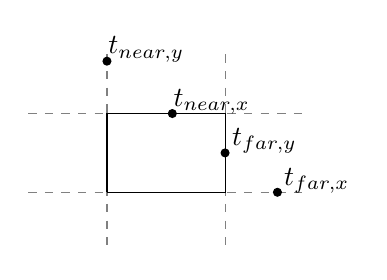
\begin{tikzpicture}[y=0.5cm, x=.5cm,font=\sffamily]
      % Planes
      \draw[dashed, color=gray] (-2,0) -- (5,0);
      \draw[dashed, color=gray] (-2,2) -- (5,2);
      \draw[dashed, color=gray] (0,3.5) -- (0,-1.5);
      \draw[dashed, color=gray] (3,3.5) -- (3,-1.5);

      % AABB
      \draw (0,0) -- (3,0) -- (3,2) -- (0,2) -- (0,0);

      % Ray
      \drawRay{-1,4}{7,-2}

      % Intersection
      \draw[fill=black] (0,3.33) circle (0.05cm);
      \draw (1,3.63) node{$t_{near,y}$};
      \draw[fill=black] (1.66,2) circle (0.05cm);
      \draw (2.66,2.3) node{$t_{near,x}$};
      \draw[fill=black] (3,1) circle (0.05cm);
      \draw (4,1.3) node{$t_{far,y}$};
      \draw[fill=black] (4.33,0) circle (0.05cm);
      \draw (5.33,0.3) node{$t_{far,x}$};

    \end{tikzpicture}
  }
  \caption{Ray/Box intersection.}
  \label{fig:rayBoxIntersection}
\end{figure}

Clearly kd-trees provide the simplest distance calculations of the
above given examples.

% Example of kd-tree flexibility over octree (important in sparse
% scenes / empty space partitioning)

Binary trees, such as kd- and bsp trees, are also more flexible than
\textit{quadtress} or \textit{octrees}, which subdivides the geometry
with 2 or 3 planes respectively per node. An example can be seen on
\reffig{fig:binQuadSplit}. This flexibility can be extremely important
when accelerating sparse scenes.

\fixme{include trees in the bsp/quad figure}

\begin{figure}
  \centering
  \subfloat[Possible binary splits.]{
    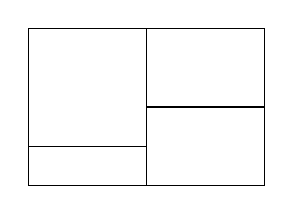
\begin{tikzpicture}[y=0.5cm, x=.5cm,font=\sffamily]
      
      % AABB
      \draw (0,0) -- (6,0) -- (6,4) -- (0,4) -- (0,0);
      
      % TRIS
      \drawTri{0,4}{3,3}{1.5,1}
      \drawTri{6,1}{4, 2}{4,0}
      
      % splits
      \draw (3,0) -- (3,4);
      \draw (0,1) -- (3,1);
      \draw (3,2) -- (6,2);
      
    \end{tikzpicture}
    \label{fig:binarySplit}
  }
  \hspace{20pt}
  \subfloat[Possible quadternary splits.]{
    \begin{tikzpicture}[y=0.5cm, x=.5cm,font=\sffamily]
      
      % AABB
      \draw (0,0) -- (6,0) -- (6,4) -- (0,4) -- (0,0);
      
      % TRIS
      \drawTri{0,4}{3,3}{1.5,1}
      \drawTri{6,1}{4, 2}{4,0}
      
      % splits
      \draw (3,0) -- (3,4);
      \draw (0,1) -- (6,1);
      
    \end{tikzpicture}
    \label{fig:quadternarySplit}
  }

  \parbox{9cm}{\caption[Comparisson of binary and quadternary
      splitting]{A comparisson of binary and quadternary
      splitting. Notice that the binary splitting planes can be placed
      without intersecting any geometry.}\label{fig:binQuadSplit}}
\end{figure}

% Vlastimil Havran did an extensive study of available spatial
% subdivision schemes (including regular grids, nested grids, octrees
% and kd-trees) and concludes in his phd thesis that kd-trees are
% better than the other schemes in most cases.

Finally, in his phd. dissertation, Vlastimil Havran did an extensive
study of spatial data structures, including grids, octress and
kd-trees, and found that the kd-tree performed the best in most cases.

Given all of the above and with the recent paper by \zhou{}, in which
kd-trees are constructed in real-time on graphics hardware, it is easy
to see why the choice fell on kd-trees as the acceleration structure.

% About this Chapter. Start by motivation. Then explain how kd-trees
% are constructed, including different strategies for choosing the
% spliting plane and doing the actual geometry splitting. Then the
% chapter will end with a discussion of how to implement the
% algorithms efficiently on a SIMT architecture.

In the rest of this chapter, we will first examine how kd-trees are
built. In particular different algorithms for choosing the splitting
plane candidate will be studied and how to handle geometry
intersecting the splitting plane will be discussed. The latter part of
this chapter deals with converting a sequential kd-tree construction
algorithm into a dataparallel algorithm. Focus is split between upper
tree nodes and lower tree nodes, once the number of geometric
primitives per node goes below a certain threshold.

\section{Building KD-trees}

A kd-tree is a binary tree that recursively subdivides geometry into
smaller tree nodes. \refalg{alg:kdTreeCreator} describes a generel
recursive kd-tree construction scheme.

\begin{algorithm}
  \caption{Recursive kd-tree constructor}
  \label{alg:kdTreeCreator}
  \begin{algorithmic}
    \PROCEDURE{ConstructKDTree}
              {$T$ : Triangle List; $voxel$ : AABB}
              {$node$ : KDNode}
              {\IF{IsLeaf($T, voxel$)}
                  \ASSIGN{$node$}{Leaf(T)}
                \ELSE
                  \COMMENTIT{Determining the splitting plane will be discussed in \refsection{sec:splittingPlane}}
                  \ASSIGN{$plane$}{DeterminePlane($T, voxel$)}
                  \ASSIGN{$(voxel_L, voxel_R)$}{Split($voxel, p$)}
                  \COMMENTIT{How to associate geometry with a voxel will be the topic of  \refsection{sec:splittingGeom}}
                  \ASSIGN{$T_L$}{AssociateGeometry($T, voxel_L$)}
                  \ASSIGN{$T_R$}{AssociateGeometry($T, voxel_R$)}
                  \ASSIGN{$node$}{Node($plane$, ConstructKDTree($T_L, voxel_L$), ConstructKDTree($T_R, voxel_R$))}
                \ENDIF}
  \end{algorithmic}
\end{algorithm}

ConstructKDTree takes as arguments a list of triangles and an axis
aligned bounding box defining the volume of the node. The algorithm
then checks if the triangles and bounding box satisfy the requirements
of being a leaf node. If so, then a leaf is produced and the recursion
terminates. If not, then a splitting plane, $plane$, needs to be
determined and the bounding box is divided by $plane$, producing a new
left and right axis aligned bounding box. Triangles are then
distributed to each new bounding box by an association algorithm and a
new node is created that will contain references to it's 2
children. An example of an iteration of ConstructKDTree can be seen in
\reffig{fig:kdIteration}.

\begin{figure}
  \centering \subfloat[A simple scene and it's corrosponding
    kd-tree. The entire scene is contained in the root node.]{
    \begin{tikzpicture}[y=0.5cm, x=0.5cm,font=\sffamily]
      \drawNode{0,0}{8,0}{8,6}{0,6}
      
      % Tris
      \drawTri{0,6}{1,4}{2,5}
      \draw (1,5) node{0};
      \drawTri{4,6}{3,4}{2,5}
      \draw (3,5) node{1};
      \drawTri{4,2}{5,6}{6,4}
      \draw (5,4) node{2};
      \drawTri{8,0}{7,2}{6,1}
      \draw (7,1) node{3};

      %axes
      \draw[->] (0,0) -- coordinate (x axis mid) (9,0);
      \draw[->] (0,0) -- coordinate (y axis mid) (0,7);
      %ticks
      \foreach \x in {0,2,...,9}
     		\draw (\x,1pt) -- (\x,-3pt)
			node[anchor=north] {\x};
    	\foreach \y in {0,2,...,7}
     		\draw (1pt,\y) -- (-3pt,\y) 
     			node[anchor=east] {\y}; 

      \draw (13,3) node [leaf] (0){$\begin{array}{c}0\\\{0, 1, 2, 3\}\end{array}$};
    \end{tikzpicture}
    \label{fig:simpleScene0}
  }

  \subfloat[The same scene as in \reffig{fig:simpleScene0}. The
    kd-tree has split the geometry down the middle and created 2 new
    leaf nodes. The geometry has then been associated with these 2
    leaf nodes.]{
    \begin{tikzpicture}[y=0.5cm, x=0.5cm,font=\sffamily]
      \drawNode{0,0}{8,0}{8,6}{0,6}
      
      % Tris
      \drawTri{0,6}{1,4}{2,5}
      \draw (1,5) node{0};
      \drawTri{4,6}{3,4}{2,5}
      \draw (3,5) node{1};
      \drawTri{4,2}{5,6}{6,4}
    \draw (5,4) node{2};
      \drawTri{8,0}{7,2}{6,1}
      \draw (7,1) node{3};

      % Splits
      \draw (4,0) -- (4,6);

      %axes
      \draw[->] (0,0) -- coordinate (x axis mid) (9,0);
      \draw[->] (0,0) -- coordinate (y axis mid) (0,7);
      %ticks
      \foreach \x in {0,2,...,9}
     		\draw (\x,1pt) -- (\x,-3pt)
			node[anchor=north] {\x};
      \foreach \y in {0,2,...,7}
     		\draw (1pt,\y) -- (-3pt,\y) 
     			node[anchor=east] {\y}; 

      \draw (14,4) node [node] (0){$\begin{array}{c}0\\x:4\end{array}$}
        child {node [leaf] (1) {$\begin{array}{c}1\\\{0, 1\}\end{array}$}}
        child {node [leaf] (2) {$\begin{array}{c}2\\\{2, 3\}\end{array}$}};
    \end{tikzpicture}
  }
  \caption{One iteration of the kd-tree construction algorithm.}
  \label{fig:kdIteration}
\end{figure}

% Left balanced non pointer vs pointers

In generel there are 2 ways a node can reference its child nodes. The
first is \textit{balanced trees}, where children of a node can be
addressed implicitly without the use of pointers. The reason for this
is that nodes at the same tree level are placed sequantially in
memory. The left and right child of node $n$ can then be indexed using
$2n+1$ and $2n+2$. The parent of a node is indexed with $\lceil n/2
\rceil - 1$.

% Balanced trees suck, example of partition with high density in one
% side and no triangles in other side. 

Wald et al.\citebook{wald:04:VVH} has the following to say about
balanced trees.

\quotebook{Balancing is optimal only for binary searching, and if all
  nodes have equal access probabilities. Neither of these two
  prerequisites are fulfilled for range queries (such as ray traversal
  and kNN queries), nor for unevenly distributed primitives such as
  photons or triangles.}{wald:04:VVH}

% Choose pointers as that would lead to less memory consumption and it
% places all nodes of the same level in a continues block, making it
% easier to work with them.

To avoid balanced trees we can instead use pointers to reference the
children. This allows for more flexibility when creating the tree.
Unfortunatly it also means storing more data per node and in the case
of slow memory access it could cause a memory latency
bottleneck. However, when experimenting with different techniques such
as is done in this thesis, the added flexibility can be a benefit and
in \refsection{sec:gpuEmptySpace} we shall see how this flexibility
can be used to add empty space maximizing, something that could not
have been done as unobtrusive had the tree been balanced.

% Triangle references

A kd-tree leaf node must be able to reference the triangles associated
with it. In this thesis I have choosen the convention that triangles
associated with a node must be placed sequentially in memory and
therefore a leaf need only contain the index of its first triangle and
the amount of triangles it is associated with.

\subsection{Choosing the Splitting Plane}\label{sec:splittingPlane}

% All the brilliance in KD-tree construction comes down to choosing
% the splitting plane and deciding when to stop.

Looking again at \refalg{alg:kdTreeCreator}, we can see that all the
brilliance in constructing a high quality kd-tree is knowing where to
place the splitting plane and when to end the recursion and create a
leaf.

% Different splitting planes heuristics.

In the following section 2 algorithms that solves this problem is
presented and then extended with empty space maximizing.


\subsubsection{Spatial Median}

% Split at the spatial median.

% Axis to split along can be choosen in a round robin fashion or the
% largest axis can be choosen. (Which initially minimises the surface
% of the children)

A quite simple method of choosing the splitting plane is to place it
at the spatial median of the nodes bounding box. There are 2 ways to
choose which dimensional spatial median to use. A \textit{round robin}
fashion can be used, where the dimensions are cycled every iteration;
ie. when creating the first node the plane will lie perpendicular to
the x-axis, the children will then be split along the y-axis, in the
next iteration the plane will split along the z-axis and then restart
again at x. Another way of choosing the dimension is to split along
the largest axis of the node's bounding box. This can be more costly
than the round robin approach, since the entire bounding box will have
to be calculated each iteration, but it will also produce the best
results.

The termination requirement for spatial median splitting is equally as
simple as choosing the splitting plane. If the number of triangles per
node falls below a certain threshold, iteration stops.

% Refered to as the naïve implementation in Wald07.

This method is refered to as naïve in \citebook{wald:06:NlogN} and
rightly so. Not much thought is put into the distribution of geometry
inside the bounding box. On \reffig{fig:crapMedian} an example is
given where the node is split in a non-intuitive way. Spatial median
splitting does, however, make up for its suboptimal splitting planes
by being quite fast, and I will therefore use it for creating my
kd-trees upper nodes, as is described in \refsection{sec:upperNodes}.

\begin{figure}
  \centering
  \begin{tikzpicture}[y=0.5cm, x=.5cm,font=\sffamily]
    % AABB
    \draw (0,0) -- (6,0) -- (6,4) -- (0,4) -- (0,0);

    % Tris
    \drawTri{0,0}{2,4}{4,0}
    \drawTri{5,4}{5.5,4}{5,3}
    \drawTri{5,2.5}{5.5,2.5}{5.5,3.5}
    \drawTri{5,2}{6,2}{5.5,0.5}

    % Split
    \draw (3,0) -- (3,4);
    \draw[dashed] (5,0) -- (5,4);

  \end{tikzpicture}

  \vspace{3mm}
  \parbox{5cm}{\caption[A poor split produced by median splitting.]{A
      poor split produced by median splitting. The solid line is a
      median split. The dashed one is a more optimal splitting plane,
      since it divides the large triangle from the
      small.}\label{fig:crapMedian}}
\end{figure}

\subsubsection{Surface Area Heuristic}

% SAH assumptions can be seen in Wald07

A far better splitting plane position can be obtained by applying the
\textit{surface area heuristic}, \textit{SAH}. Instead of only
considering the bounding volume surrounding the geometry, SAH
considers the entire geometry of a node. In essence SAH computes the
\textit{expected cost} of traversing a node, $N$, with child nodes $L$
and $R$.

\begin{displaymath}
  SAH(N \rightarrow \{L, R\}) = C_N + \frac{C_L A_L}{A_N} +
  \frac{C_R A_R}{A_N}
\end{displaymath}

where $C_N$ is the cost of traversing the node itself and is
independent of the splitting plane, $C_L$ is the cost of traversing
the left child node and $C_R$ is the cost of traversing the right
child node. $A_n$ is the summed surface area of all primitives in node
$n$. Choosing the best splitting plane amounts to applying SAH to all
possible splitting planes and then choosing the one with lowest
cost. Since the above cost evaluation does not take rays into account,
SAH assumes that rays are uniformly distributed, infinite lines.

SAH can also automatically determine when to stop splitting. Assuming
that the cost of intersecting a leaf is given as $C_{leaf} = |T| *
C_i$, where $|T|$ is the number of triangles and $C_i$ is the cost of
intersecting a triangle. SAH's termination criteria is then $C_{leaf}
< C_N$, i.e. SAH terminates when the cost of intersecting a leaf
becomes less than the cost of most optimal splitting plane.

% Globlly optimal is infeasable for complex scenes and instead a local
% greedy approximation is used.

Calculating a globally optimal solution using SAH is infeasable,
except for trivially simple scenes. A \textit{local greedy
  approximation} is used instead, where it is assumed that the created
child nodes are leafs. The makes the costs $C_L$ and $C_R$ equal to
the amount of primitives contained in the left and right child node.

Inspite of all the assumptions made by SAH, which in practice do not
hold, it is still considered one of the best heuristics and produces
trees of the highest quality.

% SAH calculation optimizations include axis round robin and some damn
% paper I can't remember.


\paragraph{Split Candidates}

% To avoid having to test the infinitely many splitting planes
% possible, we instead have to choose sensible planes for SAH.

As mentioned above the SAH cost needs to be calculated for
\textit{all} available splitting planes. Since there infinitely many
potential planes along either axis, we need some method to distinguish
useful split candidates from unimportant ones. That means we're only
interested in those finitely many planes where the geometry
association in the resulting left and right child nodes change.

% Take planes from bounding volumes

The obvious choice is to use the 6 planes defined by the triangles
axis aligned bounding box. While this is a simple and fast solution,
it can create a bloated tree, since triangles do not necessarily
overlap a node's bounding box, simply because its own bounding box
does. An example can be seen on \reffig{fig:aabbSplit}

\begin{figure}
  \centering
  \begin{tikzpicture}[y=0.5cm, x=.5cm,font=\sffamily]

    % AABB
    \draw (0,0) -- (5,0) -- (5,4) -- (0,4) -- (0,0);

    \drawTri{3,6}{7,2}{6,5}
    \drawAabb{3,2}{7,2}{7,6}{3,6}

  \end{tikzpicture}

  \vspace{3mm}
  \parbox{5cm}{\caption[Triangle/Node bounding box intersection.]{An
      example of how a triangles bounding box, the dashed box, can
      overlap a nodes bounding box, while the triangle itself does
      not.}\label{fig:aabbSplit}}
\end{figure}

Another problem with this approach is that bounding boxes of small
nodes may be completely contained inside the geometry's bounding box
and thus none of the planes are actually useful split
candidates. \reffig{fig:aabbContained} demonstrates this.

\begin{figure}
  \centering
  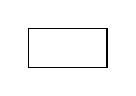
\begin{tikzpicture}[y=0.5cm, x=.5cm,font=\sffamily]

    \drawTri{0,4}{4,0}{3,3}
    \drawAabb{0,0}{4,0}{4,4}{0,4}

    % AABB
    \draw (1,1) -- (3,1) -- (3,2) -- (1,2) -- (1,1);

  \end{tikzpicture}
    
  \vspace{3mm}
  \parbox{5cm}{\caption[A tree node's bounding box contained in a
      triangle's bounding box.]{The kd-tree node's bounding box
      completely contained inside the triangles bounding
      box.}\label{fig:aabbContained}}
\end{figure}

A solution is to continuously \textit{clip} the bounding box of the
split geometry to fit the part of the geometry inside the tree nodes
bounding box, creating \textit{perfect split} condidates, as
demonstrated on \reffig{fig:aabbClipped}.

\begin{figure}
  \centering
  \begin{tikzpicture}[y=0.5cm, x=.5cm,font=\sffamily]

    \drawTri{0,4}{4,0}{3,3}
    \drawAabb{0,2}{2,2}{2,4}{0,4}
    \drawAabb{2,0}{4,0}{4,3.3}{2,3.3}

    % AABB
    \drawNode{-1,0}{2,0}{2,5}{-1,5}
    \drawNode{2,0}{5,0}{5,5}{2,5}

  \end{tikzpicture}

  \vspace{3mm}
  \parbox{5cm}{ \caption[Triangle clipping.]{The triangles bounding
      box has been clipped to fit the part of the triangle contained
      in the nodes bounding boxes.}\label{fig:aabbClipped}}
\end{figure}

Another solution is to simply remove the offending triangles, reafter
refered to as \textit{false primitives}, from the node. This can be
done by performing a triangle/box intersection check, a derivation of
the \textit{seperating axis theorem}, as described by Möller in
\citebook{Moller:2005}.


\subsubsection{Empty Space Maximizing}\label{sec:emptySpace}

An effective optimization to the quality of kd-trees is \textit{empty
  space maximization}. The idea behind the optimization is to cut away
large empty parts of the scene. This is done by placing empty leaf
nodes in the upper parts of the tree. The empty nodes will provide rays
traversing the tree with an early out option, skipping a large portion
of the geometry. 

\reffig{fig:noEmptySpaceExample} shows a simple scene without empty
space cut away and its corrosponding kd-tree. Without empty space
maximization the ray entering the scene from the lower left cornor is
forced to perform intersection test with every triangle in leaf node
1. In contrast the kd-tree in\reffig{fig:emptySpaceExample} has been
created with empty space maximization enabled and the ray entering the
scene now ends up in leaf 4. Leaf 4 is empty and allows the ray to
advance forward while skipping every triangle in leaf 1.

\begin{figure}
  \centering
  \subfloat[A simple scene without empty space cut away.]{
    \begin{tikzpicture}[y=0.5cm, x=.5cm,font=\sffamily]
      
      % AABB
      \draw (0,0) -- (10,0) -- (10,8) -- (0,8) -- (0,0);
      
      % Tris
      \drawTri{9,0}{10,2}{6,3}
      \draw (8.33,1.66) node {5};
      \drawTri{7,8}{7,4}{9,4}
      \draw (7.67,5.33) node {6};
      
      \drawTri{0,8}{0,6}{2,8}
      \draw (0.6,7.3) node {0};
      \drawTri{1,7}{0,6}{2,6}
      \draw (1,6.5) node {1};
      \drawTri{1,7}{3,6}{3,8}
      \draw (2.4,7) node {2};
      \drawTri{5,7}{3,6}{3,8}
      \draw (3.6,7) node {3};
      \drawTri{5,7}{3,6}{6,6}
      \draw (5,6.5) node {4};
      
      % Splits
      \draw (6,0) -- (6,8);
      
      % Ray
      \drawRay{0,0}{3,2}
      
    \end{tikzpicture}
    \label{fig:noEmptySpaceScene}
  }
  \hspace{5mm}
  \subfloat[The tree corrosponding to the scene in \reffig{fig:noEmptySpaceScene}.]{
    \begin{tikzpicture}[y=0.5cm, x=.5cm,font=\sffamily,
        level/.style={sibling distance=20mm/#1}]
      \node [node] {$\begin{array}{c}0\\x:6\end{array}$}
        child {node [leaf] {$\begin{array}{c}4\\\{0,1,2,3,4\}\end{array}$}}
        child {node [leaf] {$\begin{array}{c}2\\\{5, 6\}\end{array}$}};
    \end{tikzpicture}
    \label{fig:noEmptySpaceTree}
  }
  
  \caption[Scene without empty space maximization.]{A kd-tree
    constructed around a simple scene. The kd-tree doesn't use the
    empty space maximization optimization.}
  \label{fig:noEmptySpaceExample}
\end{figure}

\begin{figure}
  \centering
  \subfloat[The scene from \reffig{fig:noEmptySpaceScene} with empty space cut away.]{
    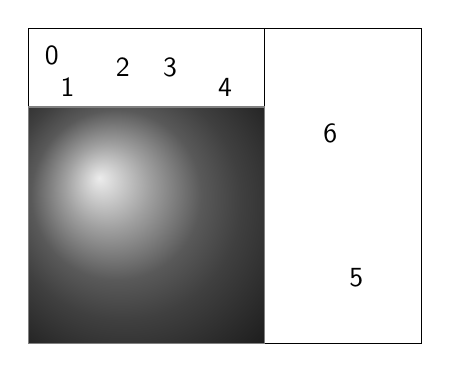
\begin{tikzpicture}[y=0.5cm, x=.5cm,font=\sffamily]
      
      % AABB
      \draw (0,0) -- (10,0) -- (10,8) -- (0,8) -- (0,0);
      
      % Tris
      \drawTri{9,0}{10,2}{6,3}
      \draw (8.33,1.66) node {5};
      \drawTri{7,8}{7,4}{9,4}
      \draw (7.67,5.33) node {6};
      
      \drawTri{0,8}{0,6}{2,8}
      \draw (0.6,7.3) node {0};
      \drawTri{1,7}{0,6}{2,6}
      \draw (1,6.5) node {1};
      \drawTri{1,7}{3,6}{3,8}
      \draw (2.4,7) node {2};
      \drawTri{5,7}{3,6}{3,8}
      \draw (3.6,7) node {3};
      \drawTri{5,7}{3,6}{6,6}
      \draw (5,6.5) node {4};
      
      % Splits
      \draw (6,0) -- (6,8);
      \draw (0,6) -- (6,6);
      
      % Empty space
      \draw[ball color=gray, color=green, shading=ball,gray] (0,0) -- (0,6) -- (6,6) -- (6,0) -- (0,0);
      
      % Ray
      \drawRay{0,0}{6,4}
      
    \end{tikzpicture}
    \label{fig:emptySpaceScene}
  }
  \hspace{5mm}
  \subfloat[The tree from \reffig{fig:noEmptySpaceTree} with the empty space nodes 3 and 4 injected.]{
    \begin{tikzpicture}[y=0.5cm, x=.5cm,font=\sffamily,
        level/.style={sibling distance=40mm/#1}]
      \node [node] {$\begin{array}{c}0\\x:6\end{array}$}
        child {node [node] {$\begin{array}{c}3\\y:6\end{array}$}
            child {node [leaf] {$\begin{array}{c}1\\\{0,1,2,3,4\}\end{array}$}}
            child {node [leaf] {$\begin{array}{c}4\\\emptyset\end{array}$}}
        }
        child {node [leaf] {$\begin{array}{c}2\\\{5, 6\}\end{array}$}};
    \end{tikzpicture}
    \label{fig:emptySpaceTree}
  }
  
  \caption[Empty space maximization.]{An example of empty space
    maximizing. The grey ball shaded area represents an empty node and
    allows the ray to leap across it and skip intersection tests with
    the 5 triangles above.}\label{fig:emptySpaceExample}
\end{figure}


Unfortunatly, how large a percentage of a node that should be empty
before empty space splitting can cut it away is highly scene specific,
making this optimization less usefull in the general case. Like \zhou{}
I have found that performing an empty space split is optimal when a
bounding box is more than 25\% empty along one of the axes.

% Dynamic empty space threshold, favor early out in the top of the tree.

% huge ray tracing performance improvement in testscene (23% without
% raytracers doing intersection tests at leaf nodes)

% Implementation is 

\subsection{Triangle/Node Association Schemes}\label{sec:splittingSchemes}

When a splitting plane has been chosen, the triangles in the split
kd-tree node needs to be associated with the two newly created leaf
nodes that they overlap. Triangles located entirely in front of the
splitting plane are associated with the left child node and triangles
entirely behind are associated with the right child node. The
association schemes discussed in this section present different
methods for handling the triangles intersected by the splitting
plane. The scheme employed is important in dynamic schemes. On one
hand a fast approximating association scheme may assign triangles to
nodes that do not necessarily contain them, resulting in larger trees
and slower ray tracing times. On the other hand a scheme rigorously
checking every triangle and only assigning triangles to nodes that
they definetly intersect will result in a smaller tree and faster ray
tracing time, but results in more time being spend creating the
acceleration structure.


%% This section will look at alternatives to triangle splitting, namely
%% \textit{triangle division}, where the triangle is not split by
%% splitting planes, but divided onto each side, by simply adjusting it's
%% bounding box, and \textit{box inclusion}, where the triangles
%% themselves are not tested for inclusion, but their bounding boxes are.

% What to do with the triangles caught in the splitting plane.


\subsubsection{Triangle splitting}

% Normally ppl split.

The most common approach when a triangle should be divided around a
splitting plane, is to actually split the triangle up into new
triangles. New triangles produced by triangle splitting will always be
located entirely within the bounding box of the kd-node they are
associated with. When performing triangle splitting there are 3 cases
to look out for, as can be seen in \reffig{fig:splittingCases}.

\begin{figure}
  \centering
  \subfloat[2 vertices to the left of the splitting plane.]{
    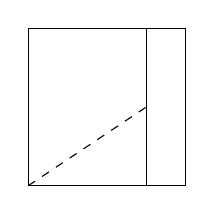
\begin{tikzpicture}[y=0.5cm, x=.5cm,font=\sffamily]
      \draw (0,0) -- (4,0) -- (4,4) -- (0,4) -- (0,0);
      \drawTri{2,4}{0,0}{4,0}
      \draw[dashed] (0,0) -- (3,2);
      \draw (3,0) -- (3,4);
    \end{tikzpicture}
    \label{fig:splittingCase1}
  }
  \hspace{5mm}
  \subfloat[1 vertex intersected by the splitting plane.]{
    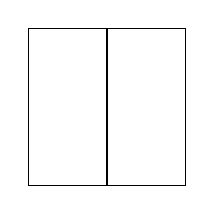
\begin{tikzpicture}[y=0.5cm, x=.5cm,font=\sffamily]
      \draw (0,0) -- (4,0) -- (4,4) -- (0,4) -- (0,0);
      \drawTri{2,4}{0,0}{4,0}
      \draw (2,0) -- (2,4);
    \end{tikzpicture}
    \label{fig:splittingCase2}
  }
  \hspace{5mm}
  \subfloat[2 vertices to the right of the splitting plane.]{
    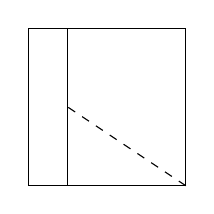
\begin{tikzpicture}[y=0.5cm, x=.5cm,font=\sffamily]
      \draw (0,0) -- (4,0) -- (4,4) -- (0,4) -- (0,0);
      \drawTri{2,4}{0,0}{4,0}
      \draw[dashed] (4,0) -- (1,2);
      \draw (1,0) -- (1,4);
    \end{tikzpicture}
    \label{fig:splittingCase3}
  }

  \vspace{3mm}
  \parbox{10cm}{\caption{The 3 different triangle splitting cases. A dashed line
      represents an additional split needed to keep representing
      geometry as triangles.}\label{fig:splittingCases}}
\end{figure}

The first case in \reffig{fig:splittingCase1} illustrates the split
when 2 vertices are located on the left of the splitting plane and one
on the right. This case is mirrored by \reffig{fig:splittingCase3}
where 2 of the vertices are located to the right of the splitting
plane. In both of these cases a triangle split will produce three new
triangles. In the last case in \reffig{fig:splittingCase2} one of the
vertices is directly intersected by the splitting plane and splits the
triangle perfectly into two new triangles. This last case however is
highly unlikely and in generel a triangle split always produces 3 new
triangles. 


\subsubsection{Triangle dividing}

\begin{figure}
  \centering
  \subfloat[One split.]{
    \begin{tikzpicture}[y=0.7cm, x=0.7cm,font=\sffamily]
      \draw (0,0) -- (4,0) -- (4,4) -- (0,4) -- (0,0);
      \drawTri{2,4}{0,0}{4,0}
      \draw[dashed] (0,0) -- (3,2);
      \draw (3,0) -- (3,4);
    \end{tikzpicture}
  }
  \subfloat[Two splits.]{
    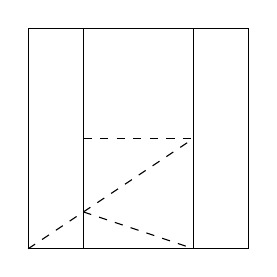
\begin{tikzpicture}[y=0.7cm, x=0.7cm,font=\sffamily]
      \draw (0,0) -- (4,0) -- (4,4) -- (0,4) -- (0,0);

      \drawTri{2,4}{0,0}{4,0}
      
      \draw (1,0) -- (1,4);
      \draw (3,0) -- (3,4);

      \draw[dashed] (1,2) -- (3,2);
      \draw[dashed] (0,0) -- (3,2);
      \draw[dashed] (1,0.667) -- (3,0);
    \end{tikzpicture}
  }
  \subfloat[Three splits.]{
    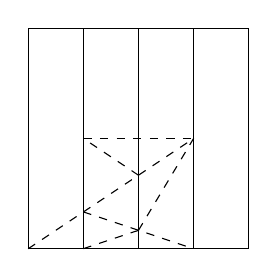
\begin{tikzpicture}[y=0.7cm, x=0.7cm,font=\sffamily]
      \draw (0,0) -- (4,0) -- (4,4) -- (0,4) -- (0,0);
      \drawTri{2,4}{0,0}{4,0}
      
      \draw (1,0) -- (1,4);
      \draw (2,0) -- (2,4);
      \draw (3,0) -- (3,4);

      \draw[dashed] (1,2) -- (3,2);
      \draw[dashed] (0,0) -- (3,2);
      \draw[dashed] (1,0.667) -- (3,0);
      \draw[dashed] (2,0.333) -- (1,0);
      \draw[dashed] (2,0.333) -- (3,2);
      \draw[dashed] (2,1.333) -- (1,2);
    \end{tikzpicture}
  }
  \caption[Excessive splitting of a triangle.]{The triangle splitting
    algorithm performing excessive splits on a triangle.}
  \label{fig:excessiveSplitting}
\end{figure}

Splitting a triangle almost always produce 3 triangles and can lead to
excessively many new triangles being created, as evidenced by
\reffig{fig:excessiveSplitting}. The problem with excessive splitting
is that each new triangle actually represents the original triangle
and so on \reffig{fig:excessiveSplitting} we see nodes containing up
to 6 triangles, all representing the exact same original and
cluttering up the tree with unnecessary geometry. A more preferable
situation is seen in \reffig{fig:dividing}, where each node only
contains one reference to the original triangle.

\begin{figure}
  \centering
  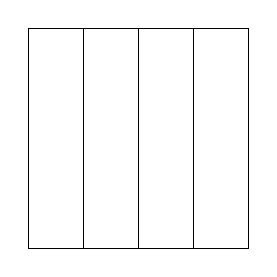
\begin{tikzpicture}[y=0.7cm, x=0.7cm,font=\sffamily]
    \draw (0,0) -- (4,0) -- (4,4) -- (0,4) -- (0,0);
    \drawTri{2,4}{0,0}{4,0}
    
    \draw (1,0) -- (1,4);
    \draw (2,0) -- (2,4);
    \draw (3,0) -- (3,4);
  \end{tikzpicture}
  
  \vspace{3mm}
  \parbox{5cm}{\caption[Dividing a triangle.]{Dividing a triangle
      among the nodes owning it. Notice that each node only contains
      one reference to the original triangle.}\label{fig:dividing}}
\end{figure}

This is the central idea behind \textit{dividing triangles}. Instead
of splitting a triangle around the splitting plane and creating new
triangles, I associated the original triangle with the new
nodes. Wether or not to associate a triangle and node is decided by
performing a \textit{triangle/bounding box overlap} test, as described
in Möller\citebook{Moller:2005}. If the triangle overlaps the child
node's bounding box after the split, then it will be associated with
that node, otherwise the triangle is excluded from the node.


\subsubsection{Box Inclusion}

% Simpler than splitting.

Performing the triangle/bounding box overlap test can be a
computationally heavy task. A cheaper splitting scheme is to test a
triangle's axis aligned bounding volume with the axis aligned bounding
volume of the node. Given that an axis aligned bounding volume, $v$,
can be described by its minimum and maximum value along each axis, I
define it as $v = \{v_{min}, v_{max}\} \in \{R^3, R^3\} $. Performing
the intersection test between the triangle's bounding volume, $t$, and
the node's, $n$, then becomes $n_{min} < v_{max} \wedge v_{min} <
n_{max}$.

\begin{figure}
  \centering
  \subfloat[]{
    \begin{tikzpicture}[y=0.5cm, x=.5cm] 
      \drawTri{1,1}{2,4}{4,3}
      \drawAabb{1,1}{1,4}{4,4}{4,1}
      
      \draw (0,0) -- (0,3) -- (3,3) -- (3,0) -- (0,0);
      \draw (3,0) -- (3,3) -- (6,3) -- (6,0) -- (3,0);
    \end{tikzpicture}
  }
  \subfloat[hut]{
    \begin{tikzpicture}[y=0.5cm, x=.5cm]
      \drawTri{1,2}{2,5}{4,4}
      \drawAabb{1,2}{1,5}{4,5}{4,2}

      \draw (0,0) -- (0,3) -- (3,3) -- (3,0) -- (0,0);
      \draw (3,0) -- (3,3) -- (6,3) -- (6,0) -- (3,0);
    \end{tikzpicture}
    \label{fig:falseBoxInclusion}
  }
  \caption{Box inclusion examples.}
  \label{fig:boxInclusion}
\end{figure}

% Naturally increases amount of \textit{false primitives} in the tree, but is
% very cheap.

\refFig{fig:boxInclusion} shows two examples of a node being split
down the middle. In both examples the triangle will be associated with
both new nodes, as the triangles bounding box overlaps both nodes. But
in \reffig{fig:falseBoxInclusion} we clearly see that the triangle
itself does not overlap the right node's bounding box. This
illustrates the drawback to only testing a triangle's bounding box and
how box inclusion will produce false positives. Triangles that do not
intersect a nodes bounding box can be associated with that node and
become a false primitive, which will increase the size of the tree and
slow down ray tracing time. However, box inclusion makes up for this
by performing fast node/triangle association, cutting down on the time
spend constructing the tree.

% Also has an increased change of looping during construction in
% combination with a small max lower size. Fx fairy forest loops using
% adjusting bounding box with a max size of 32 primtives in leaf nodes.

% False primitives can then be removed at a later stage at the cost of
% some extra overhead. Or combine with Divide every n'th step for
% optimal sweetness.

% With the added leaf intersection in the raytracer, extra triangles
% in the leaf nodes become even less important and this method starts
% to shine for dynamic scenes.






\section{Adopting the Algorithms for CUDA}

% Needs to exploit the dataparallel nature of GPU's A GPU needs as
% many of its multiprocessors occupied as possibly for optimal
% performance.

Having explored the different methods for deciding which splitting
plane to use and how to associate geometry with a node in the kd-tree,
it is time to look at the actual implementation of a kd-tree
construction algorithm on the GPU.

The generel kd-tree construction method presented in
\refalg{alg:kdTreeCreator} recursively constructs \textit{one} tree
node at a time in a \textit{depth-first} manor. In order to
efficiently utilize the GPU, as many of it's multiprocessors as
possible must be fully occupied. This means \refalg{alg:kdTreeCreator}
must be restructured to work on multiple nodes at a time. Fortunatly
this is exactly what \zhou{} did by changing the kd-tree constructor
to work on a list of nodes and recursively create the tree in
\textit{breadth-first} order, as outlines in
\refalg{alg:bfsKDTreeCreator}.

\begin{algorithm}
  \caption{BFS Recursive kd-tree constructor}
  \label{alg:bfsKDTreeCreator}
  \begin{algorithmic}
    \PROCEDURE{ConstructKDTree}
              {$activeNodes$ : Node List  \textit{\color{gray}//list of kd-nodes not processed yet}}
              {$nextNodes$ : Node List}
              {\PARALLELFOR{$node$ \textbf{in} $activeNodes$}
                 \IF{IsLeaf($node$)}
                   \ASSIGN{$node$}{Leaf($node$)}
                 \ELSE
                   \COMMENTIT{Determine the splitting plane.}
                   \ASSIGN{$plane$}{DeterminePlane($node$)}
                   \ASSIGN{$(node_L, node_R)$}{Split($node, p$)}
                   \COMMENTIT{Associate the geometry with a node and add it to the next list.}
                   \ASSIGN{$node_L.geometry$}{AssociateGeometry($node.geometry, node_L$)}
                   \STATE{$nextNodes$.Add($node_L$)}
                   \ASSIGN{$node_R.geometry$}{AssociateGeometry($node.geometry, node_R$)}
                   \STATE{$nextNodes$.Add($node_R$)}
                 \ENDIF
               \ENDFOR}
  \end{algorithmic}
\end{algorithm}

% Creating the KD-tree in BFS will optimize GPU performance at lower
% tree levels, as there would be thousands of nodes created at the
% same time.

At the lower levels, where thousands of nodes are created at a time,
breadth-first creation allows full utilization of the hardware. But
for the first levels of the tree this approach will still not fully
exploit the graphics hardware, as only a couple of nodes are active
per pass, leaving the multiprocessors underutilized.

To remedy this the tree construction will be split into 2 phases, an
upper and a lower phase. A node is said to belong to the upper part of
the tree if the number of triangles associated with it is above a
given threshold. In this thesis I will be using the thresholds 32 and
64. During the upper tree creation phase the choice of splitting plane
is parallized over all geometric primitives, of which there can be
hundreds of thousands. When creating the lower tree, there will be
thousands of nodes and computations can effectively be structured as
in \refalg{alg:bfsKDTreeCreator}.

% The structure of the rest of the chapter.

The overall construction of the tree is presented in
\refalg{alg:constructKDTree}. First the axis aligned bounding boxes of
each triangle is computed. Then the upper part of the tree is
constructed iteratively until there are no more new nodes to
process. How this is done is the topic of
\refsection{sec:upperNodes}. Once the upper part of the tree is
complete, the leaf nodes are processed and the sides of triangles'
bounding boxes are stored as potential splitting planes. The lower
part of the tree is then iteratively constructed, just as the upper
part was. \refsection{sec:lowerNodes} details 3 different algorithms
that produces lower trees with varying construction speed and quality.

\begin{algorithm}
  \caption{Construct kd-tree}
  \label{alg:constructKDTree}
  \begin{algorithmic}
    \PROCEDURE{ConstructKDTree}
              {$Triangles$ : Triangle List}
              {$root$ : Node}{
                \PARALLELFOR{$t$ \textbf{in} $Triangles$}
                  \STATE{Compute axis aligned bounding box for $t$.}
                \ENDFOR
                \STATE{}
                \DECLARE{$activeNodes, leafs, nextNodes$}{Node List}
                \COMMENTIT{Upper node construction phase.}
                \STATE{$activeNodes$.Add($rootNode$)}
                \WHILE{$activeNodes$.NotEmpty}
                  \STATE{$nextNodes$.Clear}
                  \STATE{CreateUpperNodes($activeNodes$, $leafs$, $nextNodes$)}
                  \STATE{swap($activeNodes$, $nextNodes$)}
                \ENDWHILE
                \STATE{}
                \COMMENTIT{Lower node construction phase.}
                \STATE{PreprocessLowerNodes($leafs$)}
                \STATE{CreateLowerNodes($leafs$, $activeNodes$)}
                \WHILE{$activeNodes$.NotEmpty}
                  \STATE{$nextNodes$.Clear}
                  \STATE{CreateUpperNodes($activeNodes$, $nextNodes$)}
                  \STATE{swap($activeNodes$, $nextNodes$)}
                \ENDWHILE
              }
  \end{algorithmic}
\end{algorithm}

\subsection{Upper Tree Creation}\label{sec:upperNodes}

% At upper tree level nodes exploit data parallelism by parallising
% the cost computation over triangles. 

At the uppermost levels of the kd-tree there won't be many nodes that
our computations can be parallized over. But each node can be
associated with thousands of geometric primitives and parallising the
choice of splitting plane across the geometry will utilize the GPU
effectively.

% SAH assumes that each split results in 2 leaf nodes, which is
% practically always wrong at high level nodes, therefore \zhou{}
% suggests splitting along the spatial median of the nodes longest
% axis.

The issue is then which algorithm to use when choosing the splitting
plane. SAH is a computationally heavy algorithm, since it compares
every possibly splitting plane with every triangle associated with the
node. SAH also assumes that each split results in 2 leaf nodes, which
for the upper parts of the tree is almost always wrong. This makes SAH
an undesirable algorithm for choosing the splitting plane in the upper
parts of tree, where we need to be able to efficiently decide on which
splitting plane to use. Instead \zhou{} proposes to use spatial median
splitting with empty space maximization.

The entire algorithm for constructing the upper parts of the kd-tree
can be seen in \refalg{alg:kdUpperNodeCreator}.

\begin{algorithm}
  \caption{KD-Tree upper node creator}
  \label{alg:kdUpperNodeCreator}
  \begin{algorithmic}
    \PROCEDURE{CreateUpperNodes}
               {\VAR{activeNodes} : Node List}
               {\VAR{leafs,nextNodes} : Node List}{

                 \COMMENTIT{First split all triangles into segments.}
                 \DECLARE{$segmentList$}{List}
                 \PARALLELFOR{$node$ \textbf{in} $activeNodes$}
                   \STATE{Split all triangles contained in $node$ into
                     fixed sized segments and store those in $segmentList$.}
                 \ENDFOR
                 \STATE{}
                 \COMMENTIT{Then compute each triangles bounding box
                   using reduction as described in
                   \refsection{sec:reduce}.}
                 \PARALLELFOR{$segment$ \textbf{in} $segmentList$}
                   \STATE{Compute the bounding box of the triangles in
                     each segment.}
                 \ENDFOR
                 \STATE{Using segmented reduction as described in
                   \zhou{} to compute each nodes bounding box. Perform 
                   spatial median splitting on the nodes.}

                 \STATE{}
                 \COMMENTIT{Perform empty space maximization.}
                 \COMMENTIT{See \refalg{alg:emptySpaceMaximizing}.}
                 \STATE{...}
                 \STATE{}

                 \COMMENTIT{Compute the addresses to move the
                   triangles to by comparing them to the splitting
                   plane.}
                 \DECLARE{$associateSide, associateAddr$}{List}
                 \PARALLELFOR{$segment$ \textbf{in} $segmentList$}
                   \PARALLELFOR{$triangle$ \textbf{in} $segment.triangles$}
                     \ASSIGN{$associateSide[triangle.id]$}{AssociateLeft($segment.node$, $triangle$)}
                     \ASSIGN{$associateSide[triangle.id + |triangles|]$}{AssociateRight($segment.node$, $triangle$)}
                   \ENDFOR
                 \ENDFOR
                 \ASSIGN{$associateAddr$}{\textbf{Prefix-Sum}($associateSide$)}

                 \STATE{}

                 \COMMENTIT{Split nodes.}
                 \PARALLELFOR{$node$ \textbf{in} $activeList$}
                   \STATE{Split the nodes into child
                     nodes. $associateSide$ and $associateAddr$ is
                     used to directly calculate the child nodes
                     triangle index and range.}
                   \IF{$node.child$.size < $threshold$}
                     \STATE{$leaf$.Add($node.child$)}
                   \ELSE
                     \STATE{$nextNodes$.Add($node.child$)}
                   \ENDIF
                 \ENDFOR

                 \STATE{}

                 \COMMENTIT{Move the triangles.}
                 \PARALLELFOR{$segment$ \textbf{in} $segmentList$}
                   \PARALLELFOR{$triangle$ \textbf{in} $segment.triangles$}
                     \STATE{Move the triangles to have triangles
                       associated with the same node placed
                       sequentially.}
                   \ENDFOR
                 \ENDFOR
  }
  \end{algorithmic}
\end{algorithm}

% Go over the algorithm

The algorithm takes a list of non processed nodes, $activeNodes$ as
input and returns a list of leaf nodes, $leafs$, and a list of new
nodes, $nextNodes$, that needs to be processed in the next iteration.

% Explain the overall strcuture, how the last n nodes are active
% nodes?

The nodes are placed in one large array with the structure shown in
\reffig{fig:nodeStructure}. The already processed nodes are placed in
one sequential chunk from index 0 an up. The currently active nodes
are located right after them. The child nodes created by \refalg{} is
then placed after the active nodes, with the leaf nodes to the left
and next set of active nodes to the right. This preserves the
invariant that the $n$ currently active nodes, if any, are always the
$n$ last nodes in the array after an iteration of the construction
algorithm. This is a desirable property as it means I do not need to
maintain a list of indices to active nodes, but instead I can describe
the list $activeNodes$ by a range and an index into the node
list. This also improves coalescence when subsequent threads can
access nodes sequentially.


\begin{figure}
  \centering
  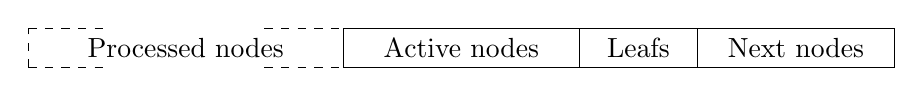
\begin{tikzpicture}[y=0.5cm, x=0.5cm]
    \draw[dashed] (0,1) -- (2,1);
    \draw[dashed] (0,0) -- (0,1);
    \draw[dashed] (0,0) -- (2,0);
    \draw (4,0.5) node {Processed nodes};
    \draw[dashed] (6,1) -- (8,1);
    \draw[dashed] (6,0) -- (8,0);
    \draw (8,1) -- (8,0);

    \draw (8,1) -- (22,1);
    \draw (8,0) -- (22,0);

    \draw (11,0.5) node {Active nodes};
    \draw (14,1) -- (14,0);

    \draw (15.5,0.5) node {Leafs};
    \draw (17,1) -- (17,0);

    \draw (19.5,0.5) node {Next nodes};
    \draw (22,1) -- (22,0);

  \end{tikzpicture}
  \caption{The structure of the kd-trees nodes in memory.}
  \label{fig:nodeStructure}
\end{figure}

% Use GPU for computations and let CPU handle minor book keeping.

As described in \refsection{sec:reduce}, our reduction algorithm
assumes that the length of the input list is a power of 2. Triangles
associated with a node are therefore split into segments with a
fixed-size that is a power of 2. Having fixed-size segments will also
make it easy to choose a kernels block size, so that each segment is
processed by one block. A segment contains information about which
triangles it contains, which node its triangles are associated with
and if there are not enough triangles to fill it, then it also stores
how many triangles it actually contains.

Performing two reductions to the triangles in the segments, once with
operator \textbf{min} and identity element $\infty$ and then with
operator \textbf{max} and identity element $-\infty$, yields the
bounding boxes of each segment. Performing a segmented reduction on
the list of segments, as describe on Algorithm 3 in \zhou, will
compute a tight bounding box for each node in activeList. This
bounding box can then be used by the spatial median splitting method
to determine where to place the splitting plane.

With the splitting plane decided for each node, the triangle/node
association can be computed by any of the methods described in
\refsection{sec:splittingSchemes}. An array of size $2 * |triangles|$,
$associateSide$, is used to store triangle/node
associations. Computing the prefix-sum of $associateSide$ will then
produce the addresses that each triangle should be moved to, in order
to be stored sequentially with the other triangles associated with the
same new node as it is.

\fixme{Example?}

%% Instead of reducing the sizes of child nodes, as done in \zhou{} I
%% propose a method for calculating them directly. This leads to lots
%% of uncoalesced lookups, so argue if the GPU is able to properly hide
%% these.

With the new addresses of the triangles computed, the nodes must now
be split into child nodes. For node $n$, the values in $associateAddr$
can be used to calculate the triangle index and range of the child
nodes, $left$ and $right$, as seen in \refalg{alg:childIndices}. The
idea behind \refalg{alg:childIndices} is that using the parent nodes
triangle index we are able to extract the triangle index of its left
and right child nodes. Then by adding the parents triangle amount to
its index, we can lookup the starting index of the next child nodes
triangles. Subtracting these two values yields the range of triangles
spanned by a child node.

\begin{algorithm}
  \caption{Compute child node triangle index and range}
  \label{alg:childIndices}
  \begin{algorithmic}
    \PROCEDURE{ChildTriangleInformation}
              {$parent, left, right$: Node, $associateAddr$ : List}
              {$left$ : Node, $right$ : Node}{
                \ASSIGN{$left.triangleIndex$}{$associateAddr[parent.triangleIndex]$}
                \ASSIGN{$leftEndAddr$}{$associateAddr[parent.triangleIndex + parent.triangleRange]$}
                \ASSIGN{$left.triangleIndex$}{$leftEndAddr - left.triangleIndex$}
                \ASSIGN{$right.triangleIndex$}{$associateAddr[parent.triangleIndex + |triangles|]$}
                \ASSIGN{$rightEndAddr$}{$associateAddr[parent.triangleIndex + parent.triangleRange]$}
                \ASSIGN{$right.triangleIndex$}{$rightEndAddr - right.triangleIndex$}
              }
  \end{algorithmic}
\end{algorithm}

Finally the triangles are moved to their new location defined by
$associateAddr$ and the algorithm has completed one iteration.





% Building the upper nodes mostly consist of moving data around, and
% not necessarily in a coalesced fashion. This makes it hard to hide
% the latency and will impact performance.

% Argue it can be done in O ( N log N )



\subsubsection{Adding empty space maximizing}\label{sec:gpuEmptySpace}

% Plugable solution, add the new nodes after the ones in nextlist.

To experiment with empty space maximization it needs to be implemented
as a plugable solution, which can be turned on and off at will. This
has been achieved with the design found in
\refalg{alg:emptySpaceMaximizing}, which injects new nodes created by
empty space maximizing into the tree. In order to perform empty space
maximizing a \textit{loose bounding box} needs to be propagated down
the tree. A loose bounding box is calculated by splitting a parents
bounding box with its splitting plane and propagated downwards to the
nodes two child nodes. Since the geometry inside a child might not
touch all sides of a parents bounding box, this propagated bounding
box provides a loose upper bound on the geometry.

\begin{algorithm}
  \caption{Calculate Empty Space Maximization}
  \label{alg:emptySpaceMaximizing}
  \begin{algorithmic}
    \PROCEDURE{CreateUpperNodes}
               {\VAR{activeNodes} : Node List}
               {\VAR{leafs,nextNodes} : Node List}{

                 \COMMENTIT{First split all triangles into segments.}
                 \STATE{...}
                 \COMMENTIT{Then compute each triangles bounding box
                   using reduction as described in
                   \refsection{sec:reduce}.}
                 \STATE{...}

                 \STATE{}
                 \COMMENTIT{Perform empty space maximization.}
                 \IF{$performEmptySpaceMaximization$}
                 \DECLARE{$emptySplitNodes, emptyAddr$}{List}
                 \DECLARE{$emptySides$}{Plane List}
                 \PARALLELFOR{$node$ \textbf{in} $activeList$}
                 \ASSIGN{$emptySplits[i]$}{$0$}
                   \FOREACH{$side$}{$node.boundingBox$}
                     \IF{$node$ has more than $C_e$ empty space on $side$}
                       \ASSIGN{$emptySplitNodes[i]$}{$emptySplitNodes[i] + 2$}
                       \STATE{$emptySides[node]$.Add($side$)}
                     \ENDIF
                   \ENDFOR
                 \ENDFOR
                 \ASSIGN{$emptyAddr$}{\textbf{Prefix-Sum}($emptySplitNodes$)}
                 \PARALLELFOR{$node$ \textbf{in} $activeList$}
                   \STATE{Cut of empty space and place new nodes
                     sequentially at addresses specified in
                     $emptyAddr$. Then rewire parent nodes to point to
                     new nodes.}
                 \ENDFOR
                 \ENDIF

                 \STATE{}
                 \COMMENTIT{Compute the addresses to move the
                   triangles to by comparing them to the splitting
                   plane.}
                 \STATE{...}
                 \COMMENTIT{Move the triangles.}
                 \STATE{...}

                 \COMMENTIT{Split nodes.}
                 \STATE{...}
  }
  \end{algorithmic}
\end{algorithm}

% Explain

The algorithm in \refalg{alg:emptySpaceMaximizing} for performing
empty space splitting is inserted right after the nodes new tight
bounding boxes have been computed and before the new child nodes are
created. If empty space maximization should be performed on one of the
nodes in activeNodes can be checked in parallel. Each side of a node
is then checked sequentially and if it is found that the amount of
empty space between the tight bounding box and the loose bounding box
on a given side is above a certain threshold, then that side is added
to the $emptySides$ list. Each empty split results in two new nodes,
one node that refers to the empty space and one node linking the
parent node with its child node. This is depicted in \reffig{TODO}.

Once the amount of empty splits per node has been decided, where to
place those nodes is computed by calculating the prefix-sum of
$emptySplitNodes$. Empty space maximization nodes are injected into to
the list of nodes shown in \reffig{fig:nodeStructure} as describe on
\reffig{fig:emptyNodeStructure}, which again preserves the invariant
that the next batch of active nodes are located at the end of the
list.

\begin{figure}
  \centering
  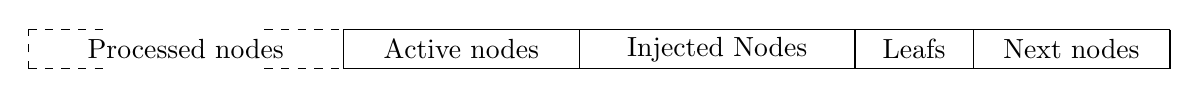
\begin{tikzpicture}[y=0.5cm, x=0.5cm]
    \draw[dashed] (0,1) -- (2,1);
    \draw[dashed] (0,0) -- (0,1);
    \draw[dashed] (0,0) -- (2,0);
    \draw (4,0.5) node {Processed nodes};
    \draw[dashed] (6,1) -- (8,1);
    \draw[dashed] (6,0) -- (8,0);
    \draw (8,1) -- (8,0);

    \draw (8,1) -- (29,1);
    \draw (8,0) -- (29,0);

    \draw (11,0.5) node {Active nodes};
    \draw (14,1) -- (14,0);

    \draw (17.5,0.5) node {Injected Nodes};
    \draw (21,1) -- (21,0);

    \draw (22.5,0.5) node {Leafs};
    \draw (24,1) -- (24,0);

    \draw (26.5,0.5) node {Next nodes};
    \draw (29,1) -- (29,0);

  \end{tikzpicture}
  \caption{The structure of the kd-trees nodes in memory with empty
    space maximization.}
  \label{fig:emptyNodeStructure}
\end{figure}


% Propagating aabb's downwards

With the addresses of the nodes produced by empty space maximization
computed, a kernel can be launched that creates the actual empty space
nodes and rewires the parent node to point to the empty space nodes
instead of its current child node. 

This construction is very flexible and all copmutations needed by
empty space maximization can be turned on and off at will, which
allows me to easily compare the quality and construction speed of
trees with and without this optimization.

\subsection{Lower Tree Creation}\label{sec:lowerNodes}

Compared with the upper tree creation phase, the lower tree creation
is quite simple and only requires a few kernels. 

% Example of how to store splitting planes as bitmaps

\begin{algorithm}
  \caption{Calculating splitting planes.}
  \label{alg:calcSplittingPlanes}
  \begin{algorithmic}
    \PROCEDURE{calcSplittingPlanes}
              {}
              {}{
                \STATE{hat}
              }
  \end{algorithmic}
\end{algorithm}

\subsubsection{SAH Tree}

\begin{algorithm}
  \caption{Calculate SAH cost}
  \label{alg:calcSAHCost}
  \begin{algorithmic}
    \PROCEDURE{ComputeSAHCost}
              {$activeNodes$ : Node List}
              {$splittingPlanes$ : Plane List, $leafs$ : Boolean List}{
                \COMMENTIT{Calculate SAH for each split candidate and
                  return the split candidate with minimal SAH.}
                \PARALLELFOR{node \VAR{i} \textbf{in} activeList}
                  \FOREACH{split candidate $s$}{$i.splitCandidates$}
                    \ASSIGN{$bmp_L$}{$i.triangles \cap s.left$}
                    \ASSIGN{$C_L$}{$\parallel bmp_L \parallel$}
                    \ASSIGN{$A_L$}{summed surface area of $bmp_L$}
                    \ASSIGN{$bmp_R$}{$i.triangles \cap s.right$}
                    \ASSIGN{$C_R$}{$\parallel bmp_R \parallel$}
                    \ASSIGN{$A_R$}{summed surface area of $bmp_R$}
                    \ASSIGN{$weightedArea$}{$C_L * A_L + C_R * A_R$}
                  \ENDFOR
                  \ASSIGN{$splittingPlanes[i] \leftarrow p$}{Split candidate with minimal weighted area}
                  \ASSIGN{$SAH$}{$p.weightedArea / i.summedArea + C_N$}
                  \ASSIGN{$leafs[i]$}{$SAH < C_{leaf}$}
                \ENDFOR
              }
  \end{algorithmic}
\end{algorithm}

% Explain

% Run prefix sum on leafList and use the result as addresses for the
% children.

% When moving from upper nodes to lower nodes. Calculate a new tight
% bounding box inside the modified bounding box. Then approximate the
% new surface area by the reduction in BB volume.


\subsubsection{Balanced Tree}

% SAH is slow, so explore alternatives.

% Testing shows that 'large' leaf node improves performance, cite Horn
% about why.

% Means that lower nodes will only be split 1-2 times and then
% intersected, ie the lower splitting planes don't need to be placed
% optimally.

% Introducing the balanced split.

\begin{algorithm}
  \caption{Calculate balanced split}
  \label{alg:calcBalancedCost}
  \begin{algorithmic}
    \PROCEDURE{ComputeBalancedSplit}
              {$activeNodes$ : Node List}
              {$splittingPlanes$ : Plane List, $leafs$ : Boolean List}{
                \COMMENTIT{Compute the relation between left and right
                  triangles for each split candidate and return the
                  candidate with best relation and presumably lowest
                  subtrees.}
                \PARALLELFOR{node \VAR{i} \textbf{in} activeList}
                  \ASSIGN{$p$}{$noSplitCandidate$}
                  \FOREACH{split candidate $s$}{$i.splitCandidates$}
                    \ASSIGN{$bmp_L$}{$i.triangles \cap s.left$}
                    \ASSIGN{$C_L$}{$\parallel bmp_L \parallel$}
                    \ASSIGN{$bmp_R$}{$i.triangles \cap s.right$}
                    \ASSIGN{$C_R$}{$\parallel bmp_R \parallel$}
                    \ASSIGN{$largestSubtree$}{\MAX{$C_L$}{$C_R$}}
                    \ASSIGN{$smallestSubtree$}{\MIN{$C_L$}{$C_R$}}
                    \IF{$largestSubtree < p.largestSubtree$ \textbf{or} \\
                      $(largestSubtree = p.largestSubtree$ \textbf{and} $smallestSubtree < p.smallestSubtree$}
                      \ASSIGN{$p$}{$s$}
                    \ENDIF
                  \ENDFOR
                  \ASSIGN{$splittingPlanes[i]$}{$p$}
                  \ASSIGN{$leafs[i]$}{$(p.largestSubtree + p.largestSubtree) / 2 + C_N < C_{leaf}$}
                \ENDFOR
              }
  \end{algorithmic}
\end{algorithm}

% Explain

\subsubsection{No Tree}


